\documentclass[aspectratio=169,10pt]{beamer}

% Required packages
\usepackage[utf8]{inputenc}
\usepackage[T1]{fontenc}
\usepackage{amsmath,amssymb,amsthm}
\usepackage{graphicx}
\usepackage{listings}
\usepackage{xcolor}
\usepackage{tikz}
\usetikzlibrary{positioning,arrows.meta,fit}
\usepackage{algorithm}
\usepackage{algorithmic}
\usepackage{hyperref}
\usepackage{mimic}

% Theme settings
\usetheme{Madrid}
\usecolortheme{seahorse}
\setbeamertemplate{navigation symbols}{}
\setbeamertemplate{footline}[frame number]

% Code listing configuration
\lstset{
    language=Python,
    basicstyle=\ttfamily\scriptsize,
    keywordstyle=\color{blue}\bfseries,
    stringstyle=\color{red},
    commentstyle=\color{green!60!black},
    showstringspaces=false,
    breaklines=true,
    breakatwhitespace=true,
    frame=single,
    numbers=left,
    numberstyle=\tiny\color{gray},
    xleftmargin=1em,
    framexleftmargin=1em
}

% Title page information
\title{Reinforcement Learning}
\subtitle{Lecture 10: Proximal Policy Optimization (PPO)}
\author{Taehoon Kim}
\institute{Sogang University MIMIC Lab \\ \url{https://mimic-lab.com}}
\date{Fall Semester 2025}

\begin{document}

% Slide 1: Title Page
\begin{frame}
\titlepage
\end{frame}

% Slide 2: Today's Agenda
\begin{frame}{Today's Agenda}

\begin{itemize}
\item Course recap \& PPO motivation
\item Trust region intuition for policy updates
\item PPO objective design and clipping analysis
\item Advantage estimation with GAE

\item Implement the PPO training loop
\item Extend PPO to continuous control tasks
\item Tune hyperparameters systematically
\item Debug and benchmark trained agents
\end{itemize}

\end{frame}

% Slide 3: Learning Objectives
\begin{frame}{Learning Objectives}
\textbf{By the end of this lecture, you will be able to:}

\begin{itemize}
\item \textbf{Understand} the motivation and theory behind PPO
\item \textbf{Implement} PPO with clipped surrogate objective
\item \textbf{Apply} Generalized Advantage Estimation (GAE)
\item \textbf{Extend} PPO to continuous control problems
\item \textbf{Debug} common PPO training issues
\item \textbf{Tune} hyperparameters systematically
\end{itemize}

\vspace{1em}
\textbf{Prerequisites:}
\begin{itemize}
\item Policy gradient methods (Lecture 8-9)
\item Actor-critic architectures
\item PyTorch and Gymnasium
\end{itemize}
\end{frame}

% Slide 4: Why PPO?
\begin{frame}{Why Proximal Policy Optimization?}
\textbf{Problems with Vanilla Policy Gradients:}
\begin{itemize}
\item High variance in gradient estimates
\item Unstable learning with large policy updates
\item Poor sample efficiency
\item Sensitive to hyperparameters
\end{itemize}

\vspace{1em}
\textbf{PPO Advantages:}
\begin{itemize}
\item Simple to implement and tune
\item Stable training with clipped updates
\item Good sample efficiency
\item Works on both discrete \& continuous control
\end{itemize}


\end{frame}

% Slide 5: Course Context
\begin{frame}{PPO in the RL Landscape}
\begin{center}
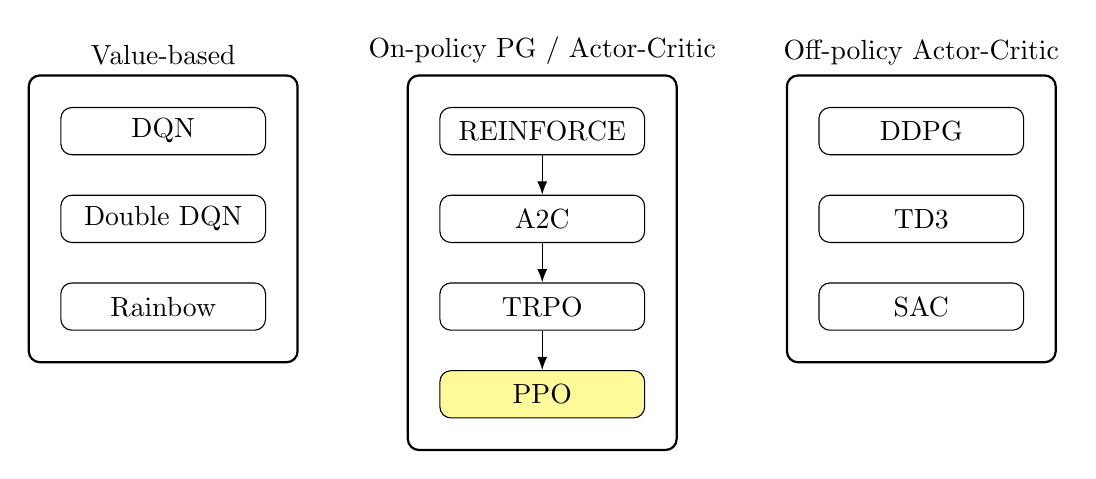
\begin{tikzpicture}[
    node distance=0.5cm,
    algo/.style={rectangle, draw, rounded corners, minimum width=2.6cm, minimum height=0.6cm, align=center},
    group/.style={rectangle, draw, thick, rounded corners, inner sep=0.4cm},
    >=Latex
]
% Value-based column
\node[algo] (dqn) {DQN};
\node[algo, below=of dqn] (ddqn) {Double DQN};
\node[algo, below=of ddqn] (rainbow) {Rainbow};
\node[group, fit=(dqn)(rainbow), label=above:Value-based] (valuegroup) {};

% On-policy PG / Actor-Critic column
\node[algo, right=2.2cm of dqn] (reinforce) {REINFORCE};
\node[algo, below=of reinforce] (a2c) {A2C};
\node[algo, below=of a2c] (trpo) {TRPO};
\node[algo, below=of trpo, fill=yellow!40] (ppo) {PPO};
\node[group, fit=(reinforce)(ppo), label=above:On-policy PG / Actor-Critic] (pggroup) {};

% Off-policy Actor-Critic column
\node[algo, right=2.2cm of reinforce] (ddpg) {DDPG};
\node[algo, below=of ddpg] (td3) {TD3};
\node[algo, below=of td3] (sac) {SAC};
\node[group, fit=(ddpg)(sac), label=above:Off-policy Actor-Critic] (acgroup) {};

% Arrows in on-policy column (historical / conceptual flow)
\draw[->] (reinforce) -- (a2c);
\draw[->] (a2c) -- (trpo);
\draw[->] (trpo) -- (ppo);

\end{tikzpicture}
\end{center}

\textbf{PPO bridges the gap:} Simple like policy gradients, stable like actor-critic
\end{frame}

% Slide 6: Policy Gradient Recap
\begin{frame}{Policy Gradient Foundation}
\textbf{Vanilla Policy Gradient (REINFORCE):}
$$\nabla_\theta J(\theta) = \mathbb{E}_{\tau \sim \pi_\theta}\left[\sum_{t=0}^{T-1} \nabla_\theta \log \pi_\theta(a_t|s_t) G_t\right]$$

\textbf{With baseline (reduces variance):}
$$\nabla_\theta J(\theta) = \mathbb{E}_{\tau \sim \pi_\theta}\left[\sum_{t=0}^{T-1} \nabla_\theta \log \pi_\theta(a_t|s_t) (G_t - b(s_t))\right]$$

\textbf{Advantage Actor-Critic:}
$$\nabla_\theta J(\theta) = \mathbb{E}_{\tau \sim \pi_\theta}\left[\sum_{t=0}^{T-1} \nabla_\theta \log \pi_\theta(a_t|s_t) A_t\right]$$

where $A_t = Q(s_t, a_t) - V(s_t)$ is the advantage function.
\end{frame}

% Slide 7: The Problem with Large Updates
\begin{frame}[fragile]{The Problem with Large Policy Updates}
\begin{columns}[T]
\begin{column}{0.5\textwidth}
\textbf{Policy Collapse Example:}

\begin{lstlisting}[basicstyle=\tiny\ttfamily]
# Large learning rate
optimizer = Adam(lr=0.1)

# One large update
loss = -log_probs * advantages
loss.backward()
optimizer.step()

# Result: Policy changes too much
# Performance drops dramatically
\end{lstlisting}

\vspace{0.5em}
\textbf{Why does this happen?}
\begin{itemize}
\item Policy distribution shifts drastically
\item Data becomes off-policy
\item Advantage estimates become invalid
\end{itemize}
\end{column}
\begin{column}{0.45\textwidth}
\textbf{Learning Rate vs Performance:}

\begin{center}
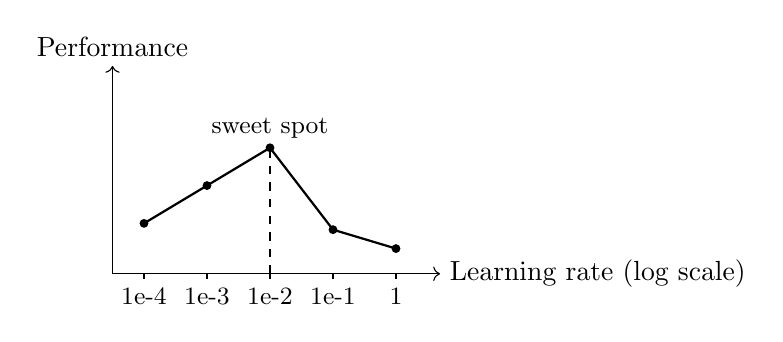
\begin{tikzpicture}[scale=0.8]
    % Axes
    \draw[->] (0,0) -- (5.2,0) node[right]{Learning rate (log scale)};
    \draw[->] (0,0) -- (0,3.3) node[above]{Performance};

    % X-axis ticks and labels (log-scale positions)
    \foreach \x/\label in {0.5/{1e-4}, 1.5/{1e-3}, 2.5/{1e-2}, 3.5/{1e-1}, 4.5/{1}}
        \draw (\x,0) -- (\x,-0.08) node[below]{\small \label};

    % Approximate performance points (scaled)
    \coordinate (p1) at (0.5,0.8);   % ~200
    \coordinate (p2) at (1.5,1.4);   % ~350
    \coordinate (p3) at (2.5,2.0);   % ~450 (peak)
    \coordinate (p4) at (3.5,0.7);   % ~100
    \coordinate (p5) at (4.5,0.4);   % ~50

    % Performance curve
    \draw[thick] (p1) -- (p2) -- (p3) -- (p4) -- (p5);

    % Points
    \foreach \pt in {p1,p2,p3,p4,p5}
        \fill (\pt) circle (2pt);

    % Annotate sweet spot
    \draw[dashed] (2.5,0) -- (2.5,2.1);
    \node[above] at (2.5,2.0) {\small sweet spot};
\end{tikzpicture}
\end{center}

\textcolor{red}{\textbf{Sweet spot exists!}}
\end{column}
\end{columns}
\end{frame}

% Slide 8: Trust Region Motivation
\begin{frame}{Trust Region Motivation}
\textbf{Key Insight:} Limit how much the policy can change in each update

\vspace{0.5em}
\textbf{Trust Region Policy Optimization (TRPO):}
$$\max_\theta \mathbb{E}_s\left[\mathbb{E}_{a \sim \pi_{\theta_{\text{old}}}}[
\frac{\pi_\theta(a|s)}{\pi_{\theta_{\text{old}}}(a|s)} A^{\pi_{\theta_{\text{old}}}}(s,a)]\right]$$

\textbf{Subject to:} $\mathbb{E}_s[D_{KL}(\pi_{\theta_{\text{old}}}(\cdot|s) || \pi_\theta(\cdot|s))] \leq \delta$

\vspace{1em}
\textbf{Problems with TRPO:}
\begin{itemize}
\item Requires second-order optimization (conjugate gradient)
\item Complex to implement correctly
\item Computationally expensive
\item Sensitive to hyperparameter $\delta$
\end{itemize}

\vspace{0.5em}
\textcolor{blue}{\textbf{PPO Solution:} Replace constraint with clipping!}
\end{frame}

% Slide 9: PPO Clipped Surrogate Objective
\begin{frame}{PPO Clipped Surrogate Objective}
\textbf{Importance sampling ratio:}
$$r_t(\theta) = \frac{\pi_\theta(a_t|s_t)}{\pi_{\theta_{\text{old}}}(a_t|s_t)}$$

\textbf{Clipped surrogate objective:}
$$L^{CLIP}(\theta) = \mathbb{E}_t\left[\min\left(r_t(\theta)A_t, \text{clip}(r_t(\theta), 1-\epsilon, 1+\epsilon)A_t\right)\right]$$

\vspace{0.5em}
\textbf{Key parameters:}
\begin{itemize}
\item $\epsilon$ (clip range): typically 0.1-0.3
\item $r_t(\theta) = 1$ when policies are identical  
\item Denominator uses fixed old policy $\pi_{\theta_{\text{old}}}$ (no gradients flow); only numerator $\pi_\theta$ is updated
\item Clipping prevents $r_t(\theta)$ from going too far from 1
\end{itemize}

\vspace{0.5em}
\textbf{Intuition:}
\begin{itemize}
\item If advantage is positive: limit how much probability can increase
\item If advantage is negative: limit how much probability can decrease
\end{itemize}
\end{frame}

% --- Inserted new frame: Clipped Objective: Case Analysis ---
\begin{frame}{Clipped Objective: Case Analysis}
\textbf{Case 1: Positive advantage ($A_t > 0$)}
\begin{itemize}
\item Objective term: $L_t^{CLIP} = \min(r_t A_t,\ \text{clip}(r_t,\ 1-\epsilon,\ 1+\epsilon)A_t)$
\item For $r_t \le 1+\epsilon$: behaves like vanilla policy gradient $r_t A_t$
\item For $r_t > 1+\epsilon$: objective becomes flat at $(1+\epsilon)A_t$
\item \textbf{Effect:} Prevents overly aggressive increases in action probability
\end{itemize}

\vspace{0.5em}
\textbf{Case 2: Negative advantage ($A_t < 0$)}
\begin{itemize}
\item For $r_t \ge 1-\epsilon$: behaves like $r_t A_t$ (reduces probability of bad actions)
\item For $r_t < 1-\epsilon$: objective becomes flat at $(1-\epsilon)A_t$
\item \textbf{Effect:} Avoids collapsing the policy by over-penalizing actions
\end{itemize}

\vspace{0.5em}
\textbf{Summary:} PPO trusts the direction of $A_t$, but only within a local window around $r_t = 1$.
\end{frame}

\begin{frame}{Understanding the Clipping Mechanism}
\begin{center}
\textbf{Clipped Surrogate for Positive vs Negative Advantage}

\vspace{1em}
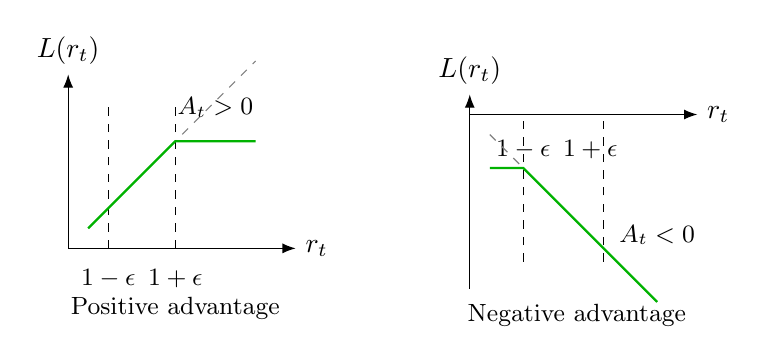
\begin{tikzpicture}[scale=0.85, >=Latex]

% ===========================
% LEFT: Positive advantage
% ===========================
\begin{scope}[shift={(-4,0)}]

    % Axes
    \draw[->] (0,0) -- (3.4,0) node[right] {$r_t$};
    \draw[->] (0,0) -- (0,2.6) node[above] {$L(r_t)$};

    % Clip boundaries
    \draw[dashed] (0.6,0) -- (0.6,2.2);
    \draw[dashed] (1.6,0) -- (1.6,2.2);

    % Move labels further down to avoid congestion
    \node[below=4pt] at (0.6,0) {\small $1-\epsilon$};
    \node[below=4pt] at (1.6,0) {\small $1+\epsilon$};

    % Unclipped line
    \draw[gray, dashed] (0.3,0.3) -- (2.8,2.8);

    % Clipped PPO objective
    \draw[thick, green!70!black]
        (0.3,0.3) --
        (1.6,1.6) --
        (2.8,1.6);

    % A_t label moved up
    \node at (2.2,2.1) {\small $A_t > 0$};

    % Caption
    \node at (1.6,-0.9) {\small Positive advantage};

\end{scope}



% ===========================
% RIGHT: Negative advantage
% ===========================
\begin{scope}[shift={(2,2)}]

    % Axes
    \draw[->] (0,0) -- (3.4,0) node[right] {$r_t$};
    \draw[->] (0,-2.6) -- (0,0.3) node[above] {$L(r_t)$};

    % Clip boundaries
    \draw[dashed] (0.8,-2.2) -- (0.8,0);
    \draw[dashed] (2.0,-2.2) -- (2.0,0);

    % Move labels down more to avoid overlap
    \node[below=6pt] at (0.8,0) {\small $1-\epsilon$};
    \node[below=6pt] at (1.8,0) {\small $1+\epsilon$};

    % Unclipped line
    \draw[gray, dashed] (0.3,-0.3) -- (2.8,-2.8);

    % Clipped PPO objective
    \draw[thick, green!70!black]
        (0.3,-0.8) --
        (0.8,-0.8) --
        (2.8,-2.8);

    % A_t label moved well above and right
    \node at (2.8,-1.8) {\small $A_t < 0$};

    % Caption
    \node at (1.6,-3.0) {\small Negative advantage};

\end{scope}

\end{tikzpicture}


\textbf{Green line = PPO objective $\min\big(r_t A_t,\ \operatorname{clip}(r_t,1-\epsilon,1+\epsilon) A_t\big)$}
\end{center}
\end{frame}
% Slide 11: Complete PPO Objective
\begin{frame}{Complete PPO Objective Function}
\textbf{Full PPO loss combines three terms:}

$$\mathcal{L}(\theta, \phi) = -\mathbb{E}_t[L^{CLIP}(\theta)] + c_v \mathbb{E}_t[L^{VF}(\phi)] - c_e \mathbb{E}_t[L^{ENT}(\theta)]$$

\vspace{0.5em}
\textbf{1. Policy Loss (Clipped):}
$$L^{CLIP}(\theta) = \min(r_t(\theta)A_t, \text{clip}(r_t(\theta), 1-\epsilon, 1+\epsilon)A_t)$$

\textbf{2. Value Function Loss:}
$$L^{VF}(\phi) = (V_\phi(s_t) - V_t^{\text{target}})^2$$

\textbf{3. Entropy Loss (exploration):}
$$L^{ENT}(\theta) = \mathbb{E}_t[\mathcal{H}(\pi_\theta(\cdot|s_t))]$$

\vspace{0.5em}
\textbf{Typical coefficients:} $c_v = 0.5$, $c_e = 0.01$
\end{frame}

% Slide 12: Value Function Clipping
\begin{frame}{Value Function Clipping (Optional)}
\textbf{Motivation:} Prevent large value function updates

\textbf{Clipped value loss:}
$$L^{VF-CLIP}(\phi) = \max\left((V_\phi(s_t) - V_t^{\text{target}})^2, (V_{\phi_{\text{old}}}(s_t) + \text{clip}(V_\phi(s_t) - V_{\phi_{\text{old}}}(s_t), -\epsilon_v, \epsilon_v) - V_t^{\text{target}})^2\right)$$

\vspace{0.5em}
\textbf{Benefits:}
\begin{itemize}
\item More stable critic learning
\item Prevents value function from changing too rapidly
\item Often improves sample efficiency
\end{itemize}

\textbf{Drawbacks:}
\begin{itemize}
\item Can slow convergence if clip range too small
\item Additional hyperparameter to tune
\end{itemize}

\vspace{0.5em}
\textbf{Common practice:} Use same $\epsilon$ for policy and value clipping
\end{frame}

% Slide 13: Generalized Advantage Estimation
\begin{frame}{Generalized Advantage Estimation (GAE)}
\textbf{Problem:} How to compute advantage $A_t = Q(s_t, a_t) - V(s_t)$?

\textbf{GAE trades off bias and variance:}
$$\hat{A}_t^{GAE(\gamma,\lambda)} = \sum_{l=0}^{\infty} (\gamma\lambda)^l \delta_{t+l}$$

where $\delta_t = r_t + \gamma V(s_{t+1}) - V(s_t)$ is the TD error.

\vspace{0.5em}
\textbf{Key parameter $\lambda$:}
\begin{itemize}
\item $\lambda = 0$: $\hat{A}_t = \delta_t$ (high bias, low variance) 
\item $\lambda = 1$: $\hat{A}_t = \sum_{k=0}^{\infty} \gamma^k r_{t+k} - V(s_t)$ (low bias, high variance)
\item $\lambda = 0.95$: Good balance (common choice)
\end{itemize}

\textbf{Recursive computation:}
$$\hat{A}_t = \delta_t + \gamma\lambda \hat{A}_{t+1}$$
\vspace{0.5em}
In practice, GAE is computed efficiently by starting at the final timestep $T$ and moving backward using this recursion.
\end{frame}

% --- Inserted new frame: GAE Example: Three-Step Trajectory ---
\begin{frame}{GAE Example: Three-Step Trajectory}
\textbf{Toy example:} 3-step episode, $\gamma = 0.9$, $\lambda = 0.9$
\begin{itemize}
\item Rewards: $r_0 = 1,\ r_1 = 1,\ r_2 = 1$
\item Value estimates: $V(s_0) = 0.5,\ V(s_1) = 0.5,\ V(s_2) = 0.5,\ V(s_3) = 0$
\end{itemize}

\textbf{Step 1: TD errors}
\[
\delta_2 = r_2 + \gamma V(s_3) - V(s_2),\ 
\delta_1 = r_1 + \gamma V(s_2) - V(s_1),\ 
\delta_0 = r_0 + \gamma V(s_1) - V(s_0)
\]

\textbf{Step 2: Backward recursion}
\[
\hat{A}_2 = \delta_2,\quad
\hat{A}_1 = \delta_1 + \gamma\lambda \hat{A}_2,\quad
\hat{A}_0 = \delta_0 + \gamma\lambda \hat{A}_1
\]

\textbf{Takeaway:} GAE mixes TD errors and multi-step returns in a simple backward pass.
\end{frame}

% Slide 14: GAE Implementation
\begin{frame}[fragile]{GAE Implementation}
\begin{lstlisting}
def compute_gae(rewards, values, dones, next_value, gamma=0.99, lam=0.95):
    """Compute Generalized Advantage Estimation"""
    advantages = []
    gae = 0
    
    # Work backwards through the episode
    for t in reversed(range(len(rewards))):
        if t == len(rewards) - 1:
            next_non_terminal = 1.0 - dones[t]
            next_value_t = next_value
        else:
            next_non_terminal = 1.0 - dones[t + 1] 
            next_value_t = values[t + 1]
        
        # TD error
        delta = rewards[t] + gamma * next_value_t * next_non_terminal - values[t]
        
        # GAE update
        gae = delta + gamma * lam * next_non_terminal * gae
        advantages.insert(0, gae)
    
    return advantages
\end{lstlisting}
\end{frame}

% Slide 15: PPO Algorithm Overview
\begin{frame}{PPO Workflow: Data Collection}
\textbf{Key loop in} \texttt{exp04\_ppo\_implementation.py}

\begin{enumerate}
    \item Initialise the policy $\pi_\theta$ and value function $V_\phi$.
    \item For each iteration:
    \begin{itemize}
        \item Roll out the current policy to gather trajectories.
        \item Compute advantages with GAE and bootstrap targets $V_t^{\text{target}}$.
        \item Normalise $\hat{A}_t$ so gradients have consistent scale.
    \end{itemize}
\end{enumerate}
\end{frame}

\begin{frame}{PPO Workflow: Optimisation Loop}
\textbf{Inner updates from} \texttt{exp04\_ppo\_implementation.py}

\begin{enumerate}
    \item Run $K$ epochs of minibatch SGD over the collected rollout batch.
    \item Evaluate ratios $r_t = \pi_\theta(a_t|s_t) / \pi_{\theta_{\text{old}}}(a_t|s_t)$.
    \item Optimise the clipped surrogate $L^{\text{CLIP}}$ plus value and entropy terms.
    \item Clip gradients (max norm 0.5) and optionally stop early when KL grows.
\end{enumerate}

\textbf{Outcome:} Stable policy improvement without large behaviour shifts.
\end{frame}

% Slide 16: Implementation Choices
\begin{frame}{Key Implementation Details}
\textbf{Critical for successful PPO training:}

\begin{columns}[T]
\begin{column}{0.48\textwidth}
\textbf{Data Collection:}
\begin{itemize}
\item Vectorized environments
\item Rollout length: 128-2048 steps
\item Batch size: num\_envs × num\_steps
\end{itemize}

\textbf{Advantage Processing:}
\begin{itemize}
\item GAE with $\lambda = 0.95$
\item Advantage normalization
\item Bootstrap from value function
\end{itemize}
\end{column}

\begin{column}{0.48\textwidth}
\textbf{Training:}
\begin{itemize}
\item Multiple epochs (4-10) per batch
\item Minibatch SGD with shuffling
\item Gradient clipping (max norm = 0.5)
\item Early stopping on KL divergence
\end{itemize}

\textbf{Hyperparameters:}
\begin{itemize}
\item Learning rate: 2.5e-4
\item Clip range: 0.2
\item Entropy coefficient: 0.01
\end{itemize}
\end{column}
\end{columns}

\vspace{0.5em}
\textcolor{red}{\textbf{Important:} These details matter greatly for performance!}
\end{frame}

% Slide 18: Implementation Session Begins
\begin{frame}{Implementation Session: PPO from Scratch}
\textbf{What we'll implement together:}

\begin{enumerate}
\item \textbf{Actor-Critic Network}
   \begin{itemize}
   \item Shared feature extractor
   \item Policy head (discrete actions)
   \item Value head
   \end{itemize}

\item \textbf{Rollout Buffer}
   \begin{itemize}
   \item Store trajectories from vectorized envs
   \item Compute GAE advantages
   \item Prepare training batches
   \end{itemize}

\item \textbf{PPO Training Loop}
   \begin{itemize}
   \item Clipped surrogate objective
   \item Multiple epochs per batch
   \item Early stopping on KL divergence
   \end{itemize}
\end{enumerate}

\textbf{Follow along:} \texttt{exp04\_ppo\_implementation.py}
\end{frame}

% Slide 19: Actor-Critic Architecture
\begin{frame}[fragile]{Actor-Critic Architecture}
\begin{lstlisting}
class ActorCritic(nn.Module):
    def __init__(self, obs_dim, act_dim, hidden_sizes=(64, 64)):
        super().__init__()

        # Shared feature extractor
        layers = []
        in_dim = obs_dim
        for hidden_dim in hidden_sizes:
            layers.extend([nn.Linear(in_dim, hidden_dim), nn.Tanh()])
            in_dim = hidden_dim
        self.feature_extractor = nn.Sequential(*layers)

        # Policy and value heads
        self.actor = nn.Linear(in_dim, act_dim)    # logits
        self.critic = nn.Linear(in_dim, 1)        # value

    def forward(self, x):
        features = self.feature_extractor(x)
        return self.actor(features), self.critic(features)
\end{lstlisting}
\end{frame}

\begin{frame}[fragile]{Actor-Critic: Sampling Utilities}
\begin{lstlisting}
class ActorCritic(nn.Module):
    ...

    def get_action_and_value(self, x):
        logits, value = self.forward(x)
        dist = torch.distributions.Categorical(logits=logits)
        action = dist.sample()
        return action, dist.log_prob(action), value
\end{lstlisting}
\textbf{Reference implementation:} \texttt{exp04\_ppo\_implementation.py}
\end{frame}

% Slide 20: Rollout Collection
\begin{frame}[fragile]{Rollout Collection (Setup)}
\begin{lstlisting}[basicstyle=\tiny\ttfamily]
def collect_rollouts(agent, envs, num_steps):
    observations, actions, logprobs, rewards, dones, values = [], [], [], [], [], []

    next_obs, _ = envs.reset()
    next_done = torch.zeros(num_envs)
    # Loop over rollout steps shown on the next slide
\end{lstlisting}
\end{frame}

\begin{frame}[fragile]{Rollout Collection (Loop)}
\begin{lstlisting}[basicstyle=\tiny\ttfamily]
    for step in range(num_steps):
        obs = next_obs

        # Get action from current policy
        with torch.no_grad():
            action, logprob, value = agent.get_action_and_value(obs)

        # Environment step
        next_obs, reward, terminated, truncated, infos = envs.step(action.numpy())
        done = np.logical_or(terminated, truncated)

        # Store step
        observations.append(obs)
        actions.append(action)
        logprobs.append(logprob)
        rewards.append(torch.tensor(reward))
        dones.append(torch.tensor(done, dtype=torch.float))
        values.append(value)

        next_obs = torch.tensor(next_obs, dtype=torch.float32)
        next_done = torch.tensor(done, dtype=torch.float32)

    return observations, actions, logprobs, rewards, dones, values, next_obs, next_done
\end{lstlisting}
\textbf{Source:} \texttt{exp04\_ppo\_implementation.py}
\end{frame}

% --- Inserted new frame: Old vs New Policy in Code ---
\begin{frame}{Old vs New Policy in Code}
\textbf{Implementing the ratio $r_t(\theta)$ in practice:}
\begin{itemize}
\item During rollout, store:
  \begin{itemize}
  \item Actions $a_t$
  \item Old log-probabilities $\log \pi_{\theta_{\text{old}}}(a_t|s_t)$ (detached)
  \item Value estimates $V_{\phi_{\text{old}}}(s_t)$
  \end{itemize}
\item During updates, recompute with the current policy:
  \begin{itemize}
  \item New logits and $\log \pi_\theta(a_t|s_t)$
  \item Ratios $r_t = \exp(\log \pi_\theta - \log \pi_{\theta_{\text{old}}})$
  \end{itemize}
\item Old values and log-probs are constants (no gradients).
\end{itemize}

\textbf{Practical tip:} Detach old log-probs in PyTorch when storing them in the rollout buffer.
\end{frame}

% Slide 21: PPO Update Step
\begin{frame}[fragile]{PPO Update (Batch Preparation)}
\begin{lstlisting}[basicstyle=\tiny\ttfamily]
def ppo_update(agent, optimizer, batch_data, clip_coef=0.2, epochs=4):
    obs, actions, old_logprobs, advantages, returns, old_values = batch_data

    # Normalize advantages
    advantages = (advantages - advantages.mean()) / (advantages.std() + 1e-8)

    for epoch in range(epochs):
        # Shuffle data
        indices = torch.randperm(len(obs))

        for start in range(0, len(obs), minibatch_size):
            end = start + minibatch_size
            mb_indices = indices[start:end]

            # Get current policy outputs
            logits, values = agent(obs[mb_indices])
            dist = torch.distributions.Categorical(logits=logits)
            new_logprobs = dist.log_prob(actions[mb_indices])
            entropy = dist.entropy().mean()
\end{lstlisting}
\end{frame}

\begin{frame}[fragile]{PPO Update (Losses \& Optimisation)}
\begin{lstlisting}[basicstyle=\tiny\ttfamily]
            # Compute ratios and losses
            ratio = torch.exp(new_logprobs - old_logprobs[mb_indices])

            # Clipped surrogate
            surr1 = ratio * advantages[mb_indices]
            surr2 = torch.clamp(ratio, 1-clip_coef, 1+clip_coef) * advantages[mb_indices]
            policy_loss = -torch.min(surr1, surr2).mean()

            # Value loss
            value_loss = F.mse_loss(values.squeeze(), returns[mb_indices])

            # Total loss
            loss = policy_loss + 0.5 * value_loss - 0.01 * entropy

            # Update
            optimizer.zero_grad()
            loss.backward()
            nn.utils.clip_grad_norm_(agent.parameters(), 0.5)
            optimizer.step()
\end{lstlisting}
\textbf{Full script:} \texttt{exp04\_ppo\_implementation.py}
\end{frame}


% Slide 23: Debugging PPO
\begin{frame}{Common PPO Issues and Debugging}
\textbf{Key metrics to monitor:}

\begin{columns}[T]
\begin{column}{0.48\textwidth}
\textbf{Policy Metrics:}
\begin{itemize}
\item KL divergence ($< 0.05$)
\item Clip fraction (0.1 - 0.3)
\item Policy entropy (decreasing)
\item Importance ratios (near 1.0)
\end{itemize}

\textbf{Training Metrics:}
\begin{itemize}
\item Gradient norms (0.1 - 10)
\item Value function error
\item Advantage statistics
\item Episode returns
\end{itemize}
\end{column}

\begin{column}{0.48\textwidth}
\textbf{Common Problems:}
\begin{itemize}
\item Too high learning rate $\rightarrow$ instability
\item Too low clip range $\rightarrow$ slow learning  
\item No entropy $\rightarrow$ premature convergence
\item Poor advantage estimation $\rightarrow$ high variance
\end{itemize}

\textbf{Debug Script:}
\texttt{exp07\_debugging\_techniques.py}
\end{column}
\end{columns}

\vspace{0.5em}
\textcolor{red}{\textbf{Rule:} Always check KL divergence and clip fraction first!}
\vspace{0.5em}
\textbf{Interpreting KL and clip fraction:}
\begin{itemize}
\item Large KL and high clip fraction → updates too aggressive; reduce learning rate or clip range
\item Very small KL and near-zero clip fraction → updates too conservative; increase learning rate or clip range
\end{itemize}
\end{frame}

% Slide 24: Continuous Control Extension
\begin{frame}{Extending PPO to Continuous Control}
\textbf{Key differences for continuous actions:}

\begin{columns}[T]
\begin{column}{0.48\textwidth}
\textbf{Discrete Actions:}
\begin{itemize}
\item Policy outputs: logits
\item Distribution: Categorical
\item Action sampling: $\text{argmax}$ or sample
\item Action space: $\{0, 1, 2, \ldots, n-1\}$
\end{itemize}

\textbf{Example environments:}
\begin{itemize}
\item CartPole-v1
\item LunarLander-v2
\item Atari games
\end{itemize}
\end{column}

\begin{column}{0.48\textwidth}
\textbf{Continuous Actions:}
\begin{itemize}
\item Policy outputs: mean, std
\item Distribution: Gaussian (Normal)
\item Action sampling: $a \sim \mathcal{N}(\mu, \sigma)$
\item Action space: $\mathbb{R}^d$ (bounded)
\end{itemize}

\textbf{Example environments:}
\begin{itemize}
\item Pendulum-v1  
\item BipedalWalker-v3
\item MuJoCo robotics
\end{itemize}
\end{column}
\end{columns}

\vspace{1em}
\textbf{Implementation:} \texttt{exp08\_continuous\_control.py}
\end{frame}

% Slide 25: Gaussian Policy Implementation
\begin{frame}[fragile]{Gaussian Policy (Network Definition)}
\begin{lstlisting}
class ContinuousActorCritic(nn.Module):
    def __init__(self, obs_dim, act_dim, hidden_sizes=(64, 64)):
        super().__init__()

        # Shared features
        self.feature_extractor = build_mlp(obs_dim, hidden_sizes)

        # Policy head - outputs mean
        self.actor_mean = nn.Linear(hidden_sizes[-1], act_dim)

        # Log standard deviation (learnable parameter)
        self.actor_logstd = nn.Parameter(torch.zeros(act_dim))

        # Value head
        self.critic = nn.Linear(hidden_sizes[-1], 1)
\end{lstlisting}
\end{frame}

\begin{frame}[fragile]{Gaussian Policy (Sampling \& Value)}
\begin{lstlisting}
class ContinuousActorCritic(nn.Module):
    ...

    def get_action_and_value(self, x, action=None):
        features = self.feature_extractor(x)

        action_mean = self.actor_mean(features)
        action_std = torch.exp(self.actor_logstd)

        # Create Gaussian distribution
        dist = torch.distributions.Normal(action_mean, action_std)

        if action is None:
            action = dist.sample()

        log_prob = dist.log_prob(action).sum(dim=-1)  # Sum over action dims
        entropy = dist.entropy().sum(dim=-1)
        value = self.critic(features).squeeze(-1)

        return action, log_prob, entropy, value
\end{lstlisting}
\textbf{Script reference:} \texttt{exp08\_continuous\_control.py}
\end{frame}

% Slide 26: Action Bounds Handling
\begin{frame}{Handling Action Bounds}
\textbf{Problem:} Most continuous environments have bounded action spaces

\textbf{Solution Options:}

\begin{enumerate}
\item \textbf{Clipping (Simple):}
   \begin{itemize}
   \item Sample from Gaussian, then clip: $a = \text{clip}(a_{\text{raw}}, a_{\min}, a_{\max})$
   \item Pro: Easy to implement
   \item Con: Breaks differentiability, can cause issues
   \end{itemize}

\item \textbf{Tanh Squashing (Better):}
   \begin{itemize}
   \item $a = \tanh(a_{\text{raw}}) \cdot \text{scale} + \text{bias}$  
   \item Include Jacobian correction in log probability
   \item Pro: Smooth, differentiable
   \item Con: Slightly more complex
   \end{itemize}
   \vspace{0.3em}
   In research and production settings, log-probability Jacobian correction is essential, but for coursework-level implementations, using tanh squashing without correction still yields reasonable performance.

\item \textbf{Beta Distribution:}
   \begin{itemize}
   \item Naturally bounded to $[0, 1]$, then rescale
   \item Pro: Theoretically clean
   \item Con: Less commonly used
   \end{itemize}
\end{enumerate}

\textbf{Recommendation:} Use tanh squashing for best results
\end{frame}



% Slide 28: Hyperparameter Sensitivity
\begin{frame}{PPO Hyperparameter Sensitivity Analysis}
\textbf{Critical hyperparameters ranked by sensitivity:}

\begin{enumerate}
\item \textbf{Learning Rate} (most sensitive)
   \begin{itemize}
   \item Range: $10^{-5}$ to $10^{-3}$
   \item Sweet spot: $2.5 \times 10^{-4}$
   \item Effect: Too high $\rightarrow$ instability, too low $\rightarrow$ slow learning
   \end{itemize}

\item \textbf{Clip Range ($\epsilon$)}
   \begin{itemize}  
   \item Range: 0.1 to 0.3
   \item Sweet spot: 0.2
   \item Effect: Too low $\rightarrow$ conservative updates, too high $\rightarrow$ instability
   \end{itemize}

\item \textbf{Batch Size (num\_envs $\times$ num\_steps)}
   \begin{itemize}
   \item Range: 512 to 8192  
   \item Sweet spot: 1024-2048
   \item Effect: Larger $\rightarrow$ more stable but less responsive
   \end{itemize}
\end{enumerate}

\textbf{Systematic tuning:} \texttt{exp06\_hyperparameter\_sensitivity.py}
\end{frame}

% Slide 29: Hyperparameter Tuning Strategy
\begin{frame}{Systematic Hyperparameter Tuning}
\textbf{Recommended tuning order:}

\begin{enumerate}
\item \textbf{Start with defaults:}
   \begin{itemize}
   \item Learning rate: 2.5e-4
   \item Clip range: 0.2  
   \item GAE lambda: 0.95
   \item Batch size: 2048
   \end{itemize}

\item \textbf{Tune learning rate first:}
   \begin{itemize}
   \item Try: [1e-4, 2.5e-4, 5e-4]
   \item Look for stable learning curves
   \end{itemize}

\item \textbf{Adjust batch size if needed:}
   \begin{itemize}
   \item Larger for more stable environments
   \item Smaller for faster iteration
   \end{itemize}

\item \textbf{Fine-tune other parameters:}
   \begin{itemize}
   \item Entropy coefficient (exploration)
   \item Number of epochs per update
   \item Value function coefficient
   \end{itemize}
\end{enumerate}

\textbf{Key principle:} Change one parameter at a time!
\end{frame}

% Slide 30: Advanced PPO Techniques
\begin{frame}{Advanced PPO Techniques}
\textbf{Performance optimizations:}

\begin{columns}[T]
\begin{column}{0.48\textwidth}
\textbf{Computational:}
\begin{itemize}
\item Vectorized environments
\item Mixed precision training (AMP)
\item torch.compile() for faster execution
\item Gradient accumulation
\end{itemize}

\textbf{Algorithmic:}
\begin{itemize}
\item Learning rate annealing
\item Reward scaling/normalization
\item Observation normalization
\item Dual clip (PPO-M)
\end{itemize}
\end{column}

\begin{column}{0.48\textwidth}
\textbf{Engineering:}
\begin{itemize}
\item Proper logging and monitoring
\item Checkpointing and resumption
\item Distributed training
\item Reproducibility measures
\end{itemize}

\textbf{Variants:}
\begin{itemize}
\item PPO with Curiosity
\item PPO with Hindsight Experience Replay
\item Recurrent PPO (for partial observability)
\end{itemize}
\end{column}
\end{columns}

\textbf{Production considerations:} Monitoring, robustness, deployment
\end{frame}

% Slide 31: Performance Benchmarks
\begin{frame}{PPO Performance Benchmarks}
\textbf{Expected performance on standard environments:}

\begin{center}
\begin{tabular}{|l|c|c|c|}
\hline
\textbf{Environment} & \textbf{PPO Score} & \textbf{Random Score} & \textbf{Timesteps} \\
\hline
CartPole-v1 & 400+ & 20 & 100K \\
LunarLander-v2 & 200+ & -150 & 500K \\
BipedalWalker-v3 & 300+ & -100 & 2M \\
Pendulum-v1 & -200 & -1500 & 200K \\
HalfCheetah-v2 & 2000+ & -300 & 2M \\
\hline
\end{tabular}
\end{center}

\textbf{Training tips for good performance:}
\begin{itemize}
\item Use multiple random seeds (3-5) for reliable results
\item Monitor clip fraction and KL divergence during training
\item Ensure entropy decreases gradually (not too fast)
\item Value function should learn to predict returns accurately
\end{itemize}

\textbf{Comparison with other algorithms:}
\begin{itemize}
\item PPO vs A2C: More stable, better sample efficiency
\item PPO vs SAC: Simpler, works well for both discrete and continuous
\item PPO vs DQN: Better for continuous control, policy-based exploration
\end{itemize}
\end{frame}

% Slide 32: Real-world Applications
\begin{frame}{PPO in the Real World: Games \& Robotics}
\textbf{Game AI:}
\begin{itemize}
\item OpenAI Five (Dota 2)
\item DeepMind AlphaStar (StarCraft II)
\item Hide-and-seek environments
\item Minecraft and other sandbox games
\end{itemize}

\textbf{Robotics:}
\begin{itemize}
\item Manipulation and grasping policies
\item Locomotion control for legged robots
\item Drone navigation and trajectory following
\item Humanoid balance and walking controllers
\end{itemize}
\end{frame}

\begin{frame}{PPO in the Real World: NLP \& Beyond}
\textbf{Language models and RLHF:}
\begin{itemize}
\item Reinforcement Learning from Human Feedback (ChatGPT, GPT-4)
\item Text summarisation and dialogue systems
\item Code generation with preference optimisation
\end{itemize}

\textbf{Other domains:}
\begin{itemize}
\item Autonomous driving and fleet control
\item Quantitative trading and resource allocation
\item Scientific discovery and experiment design
\end{itemize}

\textbf{Why PPO is popular:}
\begin{itemize}
\item Robust across diverse tasks with minimal tuning
\item Straightforward to implement and debug
\item Balanced sample efficiency and stability
\item Excellent open-source support and baselines
\end{itemize}
\vspace{0.5em}
The clipped surrogate objective and GAE you learned today are core components underlying many RLHF-style training pipelines for large language models.
\end{frame}

% Slide 33: Implementation Best Practices
\begin{frame}{Implementation Best Practices: Architecture \& Training}
\textbf{Code organization highlights:}
\begin{itemize}
    \item Choose between shared or separate actor/critic backbones.
    \item Use orthogonal weight initialisation for stability.
    \item Normalise layers or observations when gradients explode.
    \item Keep the training loop vectorised with shuffled minibatches.
    \item Stop early when KL divergence exceeds the trust-region budget.
\end{itemize}
\end{frame}

\begin{frame}{Implementation Best Practices: Monitoring \& Reliability}
\textbf{Monitor during training:}
\begin{itemize}
    \item Episode returns/lengths, policy entropy, gradient norms.
    \item Value prediction error and actual clip fraction.
\end{itemize}

\textbf{Reproducibility checklist:}
\begin{itemize}
    \item Fix random seeds and deterministic flags.
    \item Log environment versions and hyperparameters.
    \item Track experiment configs alongside checkpoints.
\end{itemize}

\textbf{Avoid these pitfalls:}
\begin{itemize}
    \item Skipping advantage normalisation or mishandling episode termini.
    \item Incorrect importance sampling ratios or too few parallel envs.
\end{itemize}
\end{frame}

% Slide 34: Comparison with Other Methods
\begin{frame}{PPO vs Other RL Algorithms}

\begin{center}
\begin{tabular}{|l|c|c|c|c|}
\hline
\textbf{Algorithm} & \textbf{Sample Eff.} & \textbf{Stability} & \textbf{Simplicity} & \textbf{Generality} \\
\hline
PPO & Good & High & High & High \\
A2C/A3C & Moderate & Moderate & High & High \\
TRPO & Good & High & Low & High \\
SAC & Very Good & High & Moderate & Moderate \\
TD3 & Very Good & High & Moderate & Low \\
DQN & Good & Moderate & Moderate & Low \\
\hline
\end{tabular}
\end{center}

\textbf{When to choose PPO:}
\begin{itemize}
\item Need both discrete and continuous control
\item Want stable, reliable training
\item Implementation simplicity is important  
\item Have sufficient computational resources for on-policy learning
\end{itemize}

\textbf{When to consider alternatives:}
\begin{itemize}
\item \textbf{SAC/TD3:} Need maximum sample efficiency for continuous control
\item \textbf{DQN:} Discrete control with very limited compute
\item \textbf{TRPO:} Need theoretical guarantees (research)
\end{itemize}
\end{frame}

% Slide 35: Final Integration Session
\begin{frame}{Final Integration and Testing}
\textbf{Let's build a complete PPO system:}

\vspace{1em}
\textbf{File:} \texttt{exp09\_final\_integration.py}

\vspace{1em}
\textbf{Features we'll implement:}
\begin{enumerate}
\item Unified PPO class supporting discrete and continuous control
\item Comprehensive benchmarking suite
\item Hyperparameter sensitivity analysis
\item Model saving and loading
\item Performance visualization
\item Reproducibility testing
\end{enumerate}

\vspace{1em}
\textbf{Environments we'll test:}
\begin{itemize}
\item CartPole-v1 (discrete, simple)
\item Pendulum-v1 (continuous, simple)  
\item LunarLander-v2 (discrete, complex)
\end{itemize}

\vspace{0.5em}
\textcolor{blue}{\textbf{Goal:} Production-ready PPO implementation}
\end{frame}

% Slide 36: Benchmarking Results
\begin{frame}{Live Benchmarking Results}
\textbf{Running comprehensive benchmark...}

\vspace{1em}
\textbf{Metrics we're tracking:}
\begin{itemize}
\item Final episode return (mean $\pm$ std over multiple seeds)
\item Training stability (coefficient of variation)
\item Sample efficiency (timesteps to reach threshold)
\item Wall-clock training time
\end{itemize}

\vspace{1em}
\textbf{Quality checks:}
\begin{itemize}
\item Reproducibility across random seeds
\item Monotonic improvement in early training
\item Reasonable final performance vs literature
\item Stable convergence (no catastrophic forgetting)
\end{itemize}

\vspace{1em}
\textbf{Expected results:}
\begin{itemize}
\item CartPole: $450 \pm 50$ (out of 500 max)
\item Pendulum: $-200 \pm 50$ (higher is better)
\end{itemize}
\end{frame}

% Slide 37: Troubleshooting Session
\begin{frame}{Troubleshooting Common Issues}
\textbf{Let's debug together:}

\vspace{1em}
\textbf{Scenario 1:} Policy not learning (flat learning curve)
\begin{itemize}
\item Check: Learning rate too low, entropy too high, poor advantage estimation
\item Debug: Monitor KL divergence, clip fraction, gradient norms
\end{itemize}

\textbf{Scenario 2:} Training unstable (high variance)
\begin{itemize}
\item Check: Learning rate too high, batch size too small, no advantage normalization
\item Debug: Plot importance sampling ratios, value function accuracy
\end{itemize}

\textbf{Scenario 3:} Good training, poor evaluation
\begin{itemize}
\item Check: Overfitting, environment randomization, evaluation protocol
\item Debug: Compare training vs evaluation environments
\end{itemize}

\vspace{1em}
\textbf{Debug script:} \texttt{exp07\_debugging\_techniques.py}
\end{frame}

% Slide 38: Extensions and Variants
\begin{frame}{PPO Extensions and Research Directions}
\textbf{Active research areas:}

\begin{columns}[T]
\begin{column}{0.48\textwidth}
\textbf{Algorithmic improvements:}
\begin{itemize}
\item PPO with KL warmup
\item Adaptive clipping schedules
\item Multi-step returns
\item Curiosity-driven exploration
\end{itemize}

\textbf{Scalability:}
\begin{itemize}
\item Distributed PPO
\item GPU-accelerated environments
\item Large batch training
\item Mixture of experts policies
\end{itemize}
\end{column}

\begin{column}{0.48\textwidth}
\textbf{Applications:}
\begin{itemize}
\item Multi-agent PPO (MAPPO)
\item Hierarchical PPO
\item Meta-learning with PPO
\item Safe reinforcement learning
\end{itemize}

\textbf{Theoretical analysis:}
\begin{itemize}
\item Convergence guarantees
\item Sample complexity bounds  
\item Policy improvement theory
\item Connection to natural gradients
\end{itemize}
\end{column}
\end{columns}

\end{frame}

% Slide 40: Key Takeaways
\begin{frame}{Key Takeaways from This Lecture}
\textbf{Theoretical insights:}
\begin{itemize}
\item PPO elegantly solves trust region optimization with simple clipping
\item GAE provides excellent bias-variance tradeoff for advantage estimation
\item Importance sampling enables off-policy-like efficiency with on-policy data
\end{itemize}

\textbf{Practical skills:}
\begin{itemize}
\item How to implement production-ready PPO from scratch
\item Debugging techniques using KL divergence and clip fraction
\item Extension to continuous control with Gaussian policies
\item Systematic hyperparameter tuning methodology
\end{itemize}

\textbf{Implementation details matter:}
\begin{itemize}
\item Advantage normalization is crucial for stability  
\item Multiple epochs per batch improves sample efficiency
\item Proper environment vectorization enables fast training
\item Early stopping prevents policy degradation
\end{itemize}
\end{frame}

% Slide 41: Next Week Preview
\begin{frame}{Next Week: Advanced Policy Methods}
\textbf{Lecture 11 Preview - Advanced Policy Optimization}

\begin{columns}[T]
\begin{column}{0.48\textwidth}
\textbf{Topics we'll cover:}
\begin{itemize}
\item RLHF and DPO for language models
\item Multi-agent PPO (MAPPO)
\item Monte Carlo Tree Search (MCTS)
\item AlphaZero and MuZero
\end{itemize}

\textbf{Applications:}
\begin{itemize}  
\item ChatGPT training pipeline
\item Game AI (chess, Go, poker)
\item Strategic decision making
\item Planning with learned models
\end{itemize}
\end{column}

\begin{column}{0.48\textwidth}
\textbf{Prerequisites for next week:}
\begin{itemize}
\item Complete today's lab exercises
\item Solid understanding of PPO
\item Familiarity with transformer architectures (helpful)
\end{itemize}

\textbf{Preparation:}
\begin{itemize}
\item Review RLHF paper (Christiano et al.)
\item Install transformers library
\item Practice PPO debugging
\end{itemize}
\end{column}
\end{columns}

\vspace{1em}
\textcolor{blue}{\textbf{Building towards:} Complete RL practitioner skillset}
\end{frame}




% Slide 44: Final Summary
\begin{frame}{Lecture 10 Summary}
\textbf{What we accomplished today:}

\begin{enumerate}
\item \textbf{Theory:} Understood PPO's clipped surrogate objective and GAE
\item \textbf{Implementation:} Built PPO from scratch with proper components
\item \textbf{Extensions:} Extended to continuous control with Gaussian policies
\item \textbf{Debugging:} Learned systematic debugging and monitoring techniques  
\item \textbf{Optimization:} Applied hyperparameter tuning and performance optimization
\item \textbf{Integration:} Created production-ready PPO with benchmarking
\end{enumerate}

\vspace{1em}
\textbf{You now have:}
\begin{itemize}
\item Deep understanding of modern policy optimization
\item Practical implementation skills for real projects
\item Debugging toolkit for reliable training
\item Foundation for advanced RL methods
\end{itemize}

\vspace{0.5em}
\textcolor{blue}{\textbf{Ready to tackle complex RL challenges!}}
\end{frame}

\end{document}
